\documentclass{beamer}
\usetheme{Madrid}

\setbeamertemplate{title page}{
  \vbox{}
  \vfill
  \begingroup
    \centering
    \usebeamertemplate{title}
    \usebeamertemplate{author}
    \vskip1.5em
    \usebeamertemplate{date}
    \vskip1.5em
    \usebeamertemplate{institute}
    \usebeamertemplate{titlegraphic}
  \endgroup
  \vfill
}


\title{Parton evolution: the energy behavior of the building blocks of matter}
\subtitle{Physics Research Showcase, 18 April, 2025}
\author{Casey Hampson}
\addtobeamertemplate{author}{}{Supervisor: Dr. Marco Guzzi\par}
\date{Kennesaw State University}
\institute[]{Supported by the National Science Foundation under Grant No. PHY-2412071}
\titlegraphic{
\includegraphics[width=0.1\textwidth]{./gfx/nsf-logo.png}}



\usepackage{amsmath}
\usepackage{amssymb}
\usepackage{siunitx}
\usepackage{mathtools}
\usepackage{esdiff}
\usepackage{esint}
\usepackage{bm}
\usepackage{tikz-feynman}
\usepackage{wrapfig}

\newcommand{\dd}{\mathrm{d}}
\newcommand{\vv}[1]{\mathbf{\bm{#1}}}


\begin{document}
\frame{\titlepage}



\begin{frame}
  \frametitle{Introduction}

  \begin{itemize}
  \item High-energy physics explores how the universe works at the smallest and largest possible scales.
  \item The Large Hadron Collider (LHC), the biggest particle accelerator ever built (CERN, Geneva, Switzerland), provides 
  us with unique opportunities to answer some of the most fundamental questions in nature.
  \item Some of these include:
    \begin{itemize}
    \item Dark matter and dark energy
    \item Properties of the Higgs boson, discovered at CERN in 2012
    \item The origin of mass, the spin of the proton
    \item New particles and interactions
    \end{itemize}
  \end{itemize}

  \begin{figure}
    \centering
    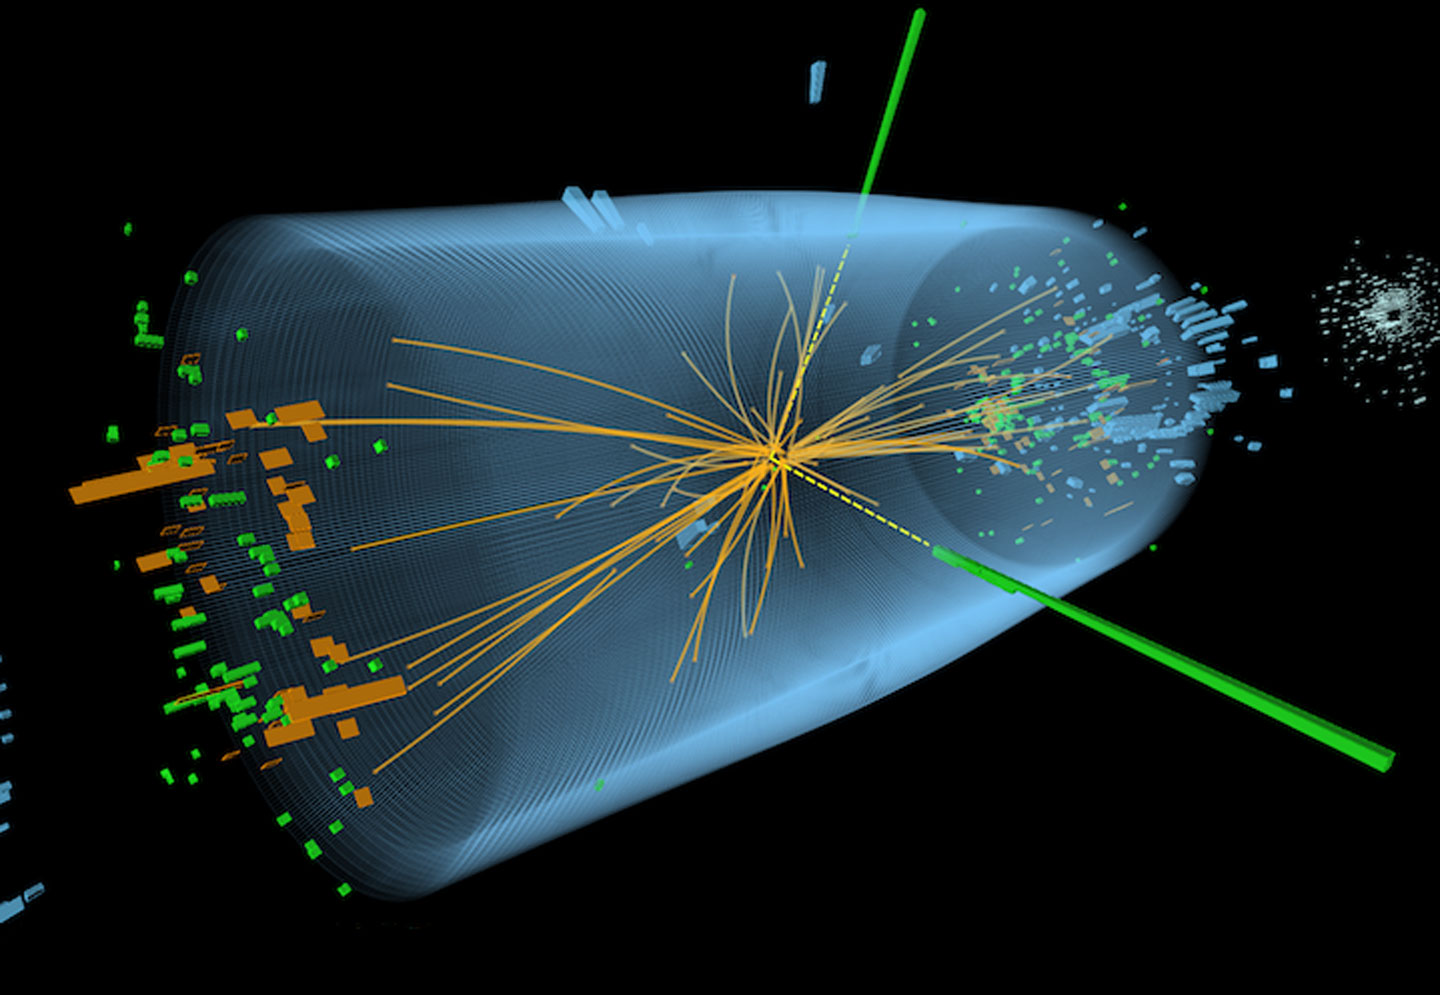
\includegraphics[width=0.35\linewidth]{./gfx/lhc.jpg}
  \end{figure}

  % maybe add another figure related to dark matter, Higgs, etc.
  
\end{frame}


\begin{frame}
  \frametitle{The CERN LHC}

  \begin{itemize}
  \item The CERN LHC collides protons 
  at nearly the speed of light around a 27Km (16.8 miles) ring at a depth of 100m (328 feet) underground.
  \item In such high-energy collisions, protons break down and a multitude of particles are produced in the final state.
  \end{itemize}

  \begin{figure}
    \centering
    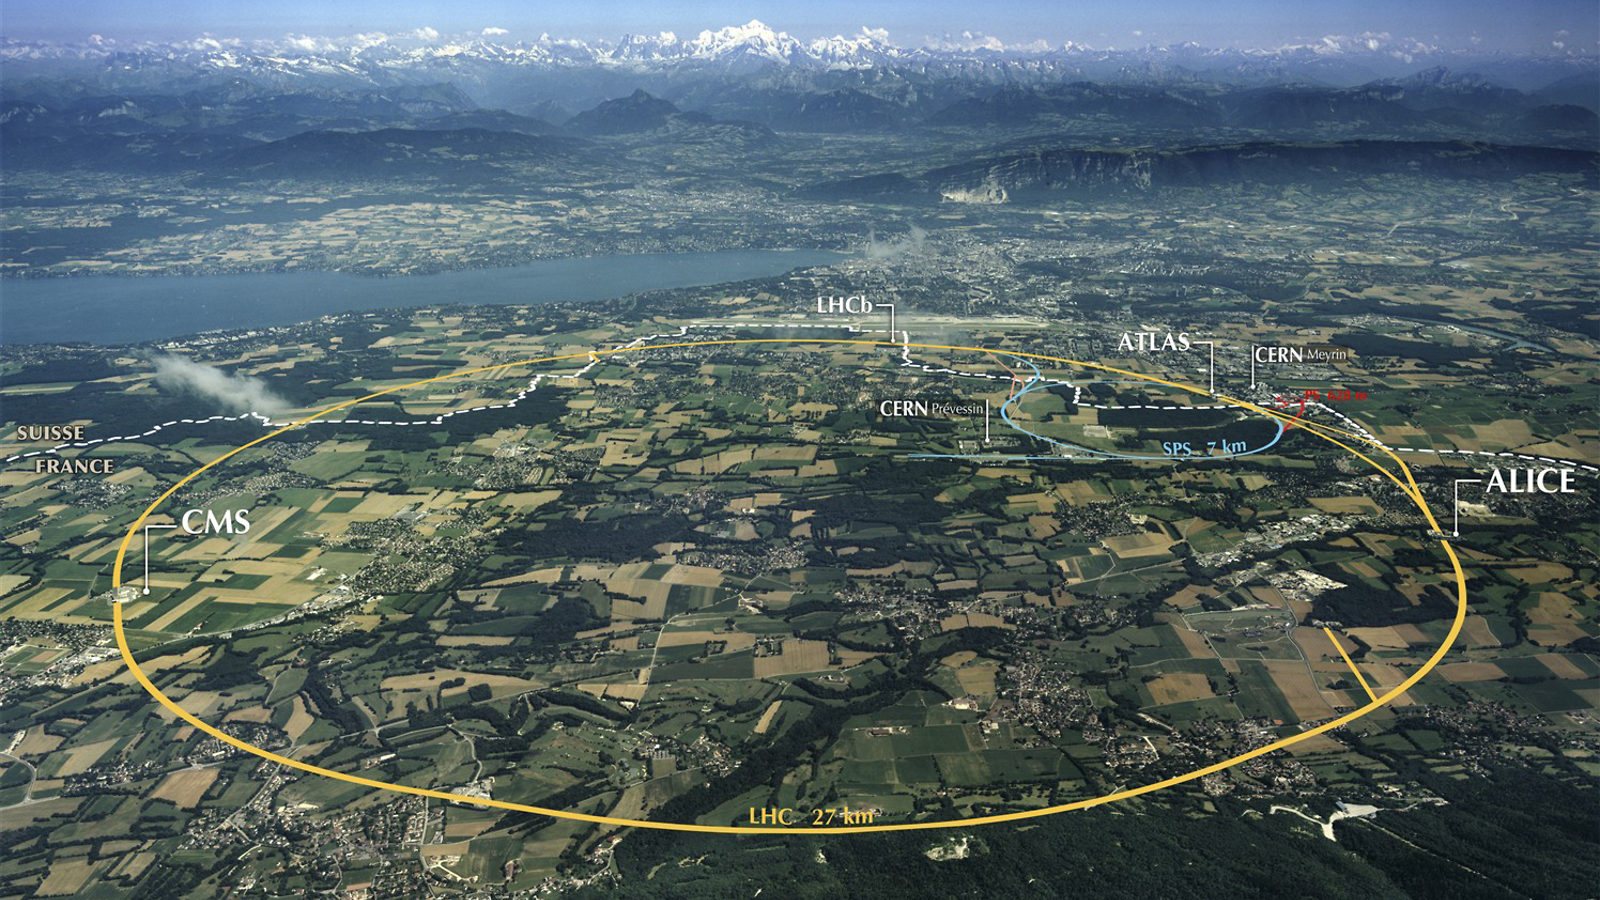
\includegraphics[width=0.7\linewidth]{./gfx/lhc-map.jpg}
  \end{figure}
\end{frame}


\begin{frame}
  \frametitle{Introduction}

  \begin{itemize}
  \item Another collider, the Electron-Ion-Collider (EIC) will be built at Brookhaven National Laboratory in the US.
  \item  LHC and EIC will complement each other and will provide us with measurements with unprecedented precision.
  \item They allow us to set stringent tests on the Standard Model and search for signatures of new physics interactions.
  \end{itemize}


  \begin{figure}
    \centering
    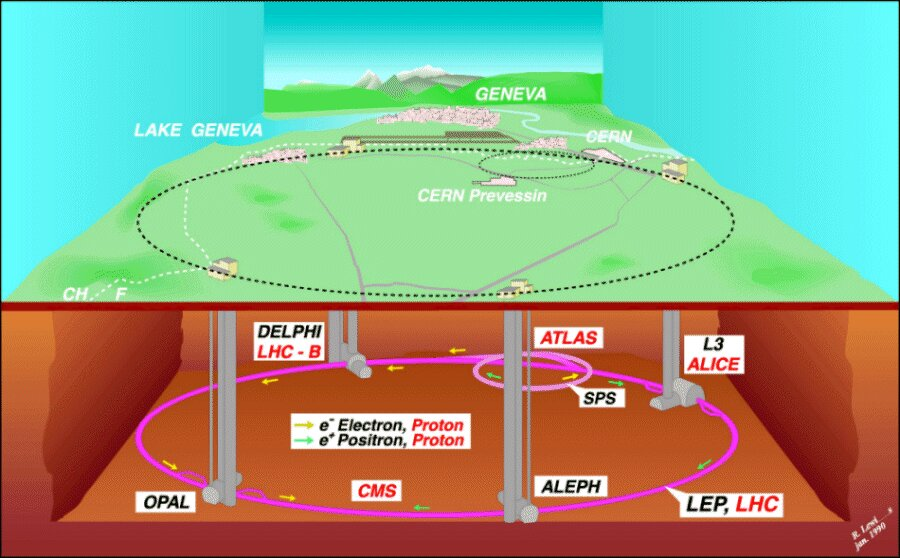
\includegraphics[width=0.44\linewidth]{./gfx/leplhc.jpg}
    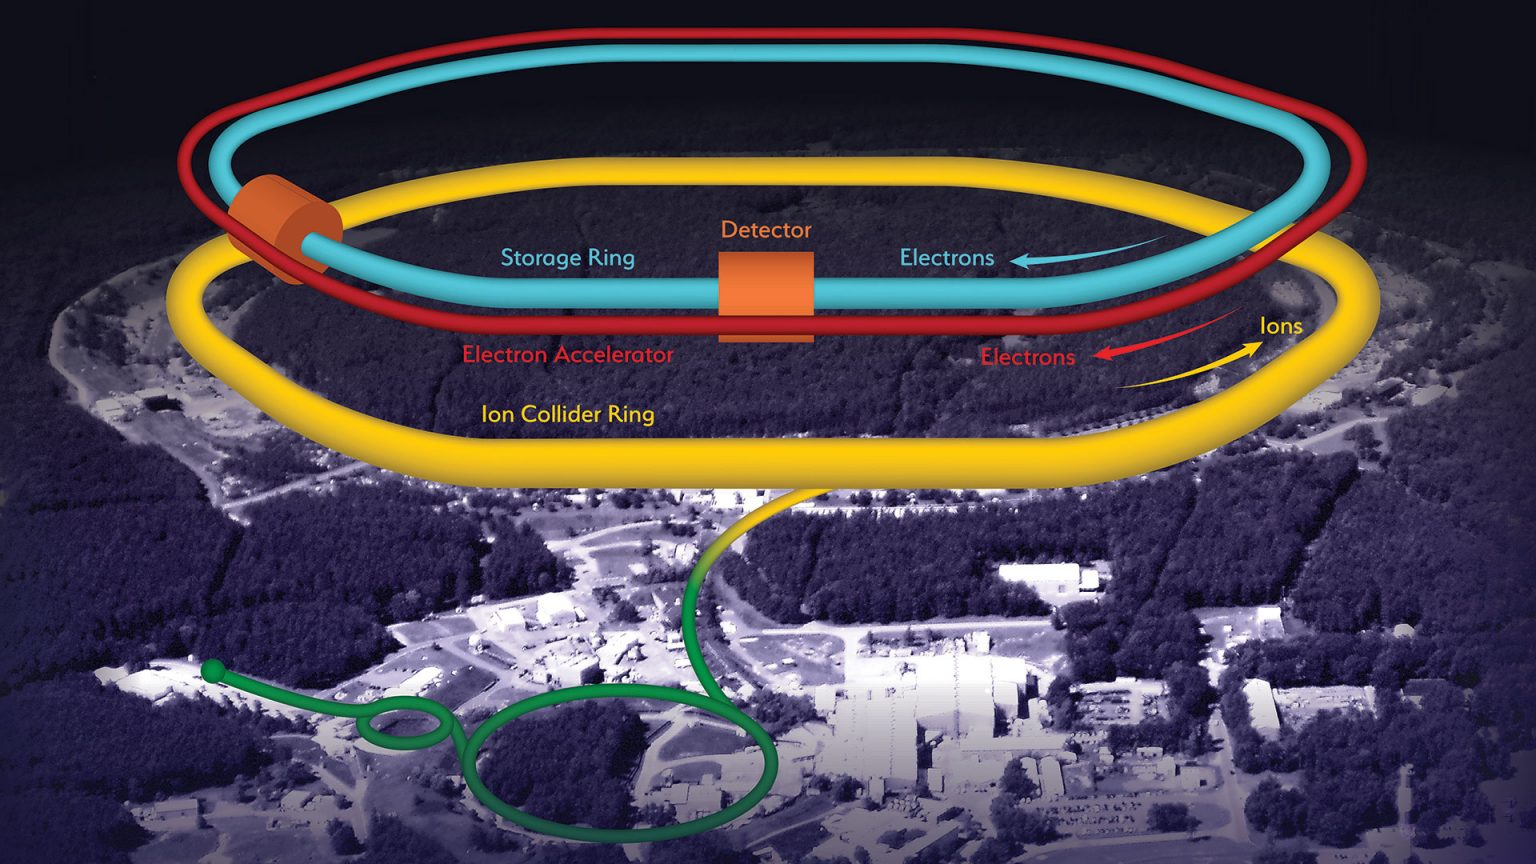
\includegraphics[width=0.44\linewidth]{./gfx/eic.jpg}
    \caption{The LHC (left); The EIC (right).}
  \end{figure}
\end{frame}


\begin{frame}
  \frametitle{The Standard Model of Elementary Particles}


  \begin{figure}
    \centering
    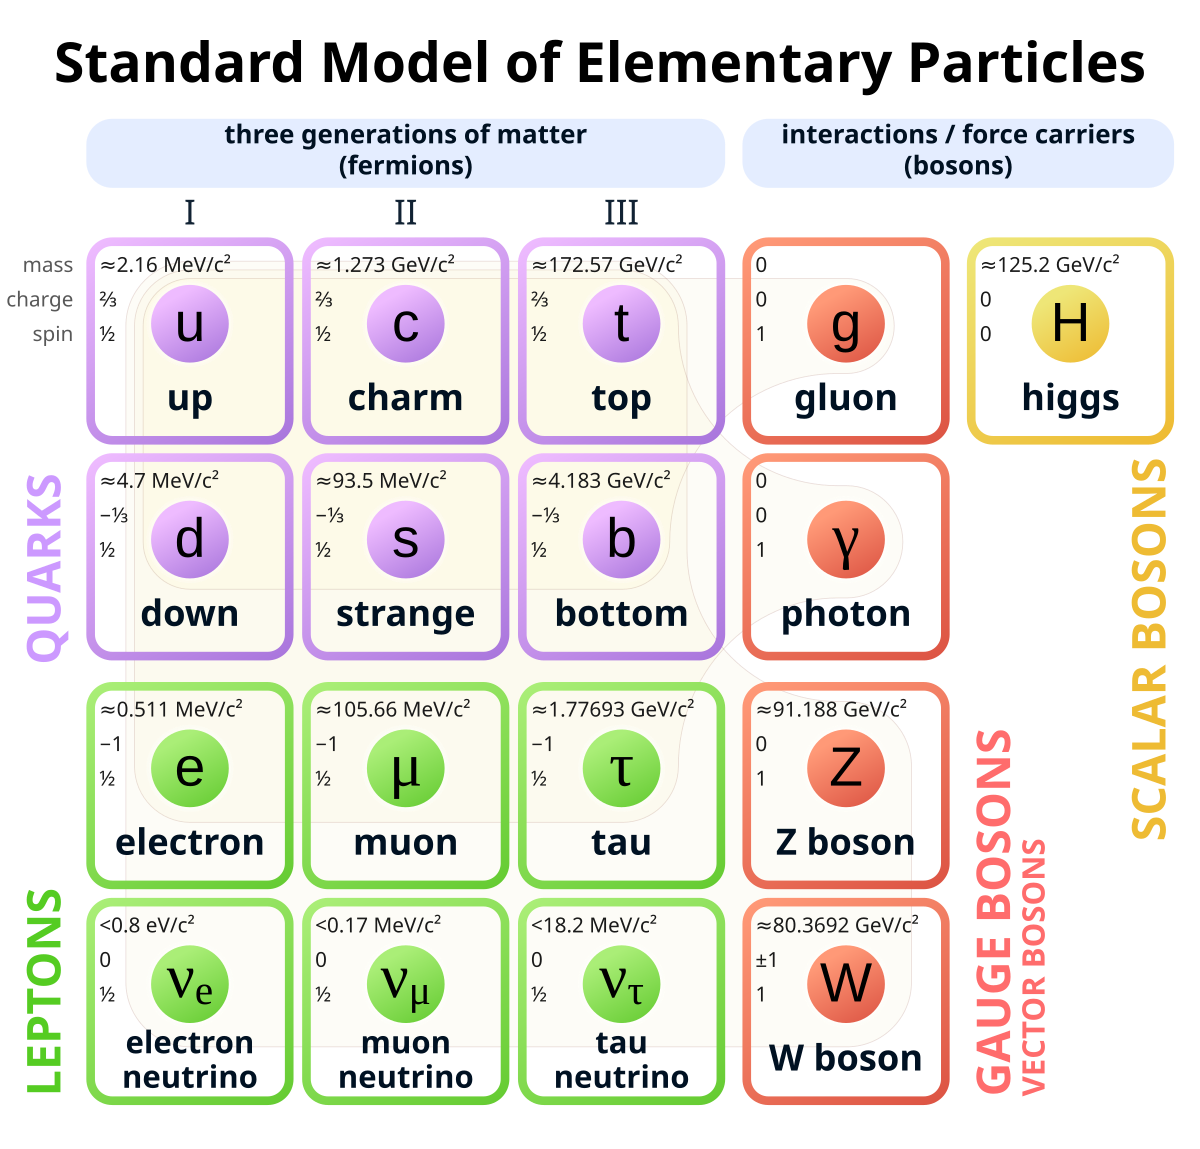
\includegraphics[width=0.4\linewidth]{./gfx/standard-model.png}
  \end{figure}

  \begin{itemize}
  \item The Standard Model is the work of decades of research and represents our best theory of fundamental interactions between particles.
  \item The Higgs boson was the most recently added particle, having been discovered in 2012 at the LHC.
  \end{itemize}

\end{frame}



\begin{frame}
  \frametitle{Photos from Summer 2024 REU at CERN}

  \begin{figure}
    \centering
    \includegraphics<1>[width=0.6\linewidth]{./gfx/cern/1.jpg}
    \includegraphics<1>[width=0.6\linewidth]{./gfx/cern/2.jpg}
    \includegraphics<2>[width=0.6\linewidth]{./gfx/cern/3.jpg}
    \includegraphics<2>[width=0.6\linewidth]{./gfx/cern/4.jpg}
  \end{figure}
  
\end{frame}


\begin{frame}
  \frametitle{The Cross Section}

  \begin{itemize}
  \item Particle colliders measure the \textbf{cross section} ($\sigma$), which is a measure of the probability that a specific process will take place in a collision. This is related to the number of events ($N_{\mathrm{ev}}$) recorded by the detectors:
 
  \begin{equation}
   \frac{N_{\mathrm{ev}}}{\mathrm{sec}} = L \cdot \sigma,
  \end{equation}

  \item $L$ is the \textbf{luminosity}, which describes the number of collisions that can be produced per $\mathrm{cm}^2$ per second.

 \item Particle theorists independently calculate $\sigma$ and compare it to experimental data.
  \end{itemize}

\end{frame}


\begin{frame}
  \frametitle{The Theoretical Cross Section}

  \begin{itemize}
  \item According to certain theorems of quantum field theory (QFT), the theoretical cross section can be written in a factorized form    
  \end{itemize}

  \begin{equation}
    \sigma = \sum_{\text{partons}=i,j} f_i \otimes f_j \otimes \hat{\sigma}_{ij} + \ldots \text{(very small/suppressed corrections)}
  \end{equation}

  \begin{itemize}
  \item $f_i$ and $f_j$ are the \textbf{parton distribution functions} (PDFs) of the proton. They represent the probability for finding a parton (quark or gluon) in the proton with a certain longitudinal momentum fraction at a particular energy scale.
  \end{itemize}
\end{frame}

\begin{frame}
  \frametitle{The Partonic Cross Section}

  \begin{itemize}
  \item $\hat{\sigma}_{ij}$ is the \textit{partonic} cross section which is perturbatively calculable and contains details of the interaction between the $i$ and $j$ partons.
  \end{itemize}

  

  \begin{figure}
    \centering
    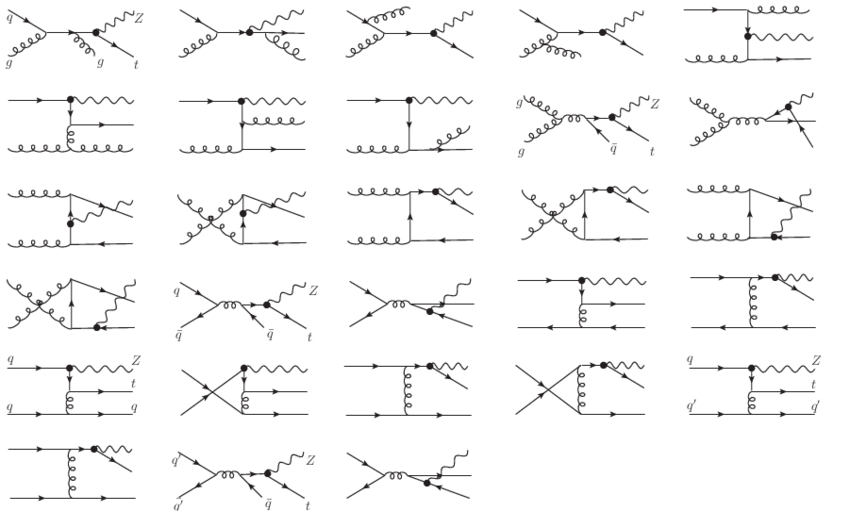
\includegraphics[width=0.7\linewidth]{./gfx/feynman-diagrams.png}
    \caption{Examples of Feynman diagrams contributing to the partonic cross section for $pp \rightarrow tZ + X$ at the LHC (Li et.al.~Phys.Rev.D.  83 (2011))}
  \end{figure}
\end{frame}


\begin{frame}
  \frametitle{What happens in proton-proton collisions?}

  \begin{itemize}
  \item At high speeds, due to special relativity, the protons get length contracted and appear as disks
  \item The inner constituents are spread throughout the disk and collide with those of the other length-contracted proton.
  \end{itemize}

  \begin{figure}
    \centering
    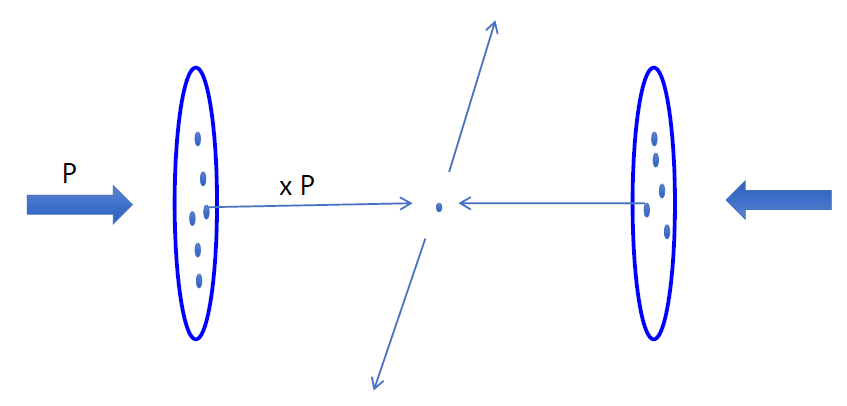
\includegraphics[width=0.6\linewidth]{./gfx/colliding-protons.png}
  \end{figure}

  \begin{itemize}
  \item PDFs map out the longitudinal momentum fractions carried by the partons in a collision.
  \end{itemize}
\end{frame}



\begin{frame}
\frametitle{Parton Distribution Functions}

\begin{itemize}
\item PDFs cannot be computed from first principles, but must be extracted from global analyses of a multitude of experiments.
\item However, given a PDF at an initial energy scale $Q_0$, one can predict how the PDF evolves with energy and determine the distributions at another scale.
\item This energy dependence is encoded in a set of (integro-differential) equations known as Dokshitzer-Gribov-Lipatov-Altarelli-Parisi (DGLAP) equations.
\end{itemize}

\begin{figure}
  \centering
  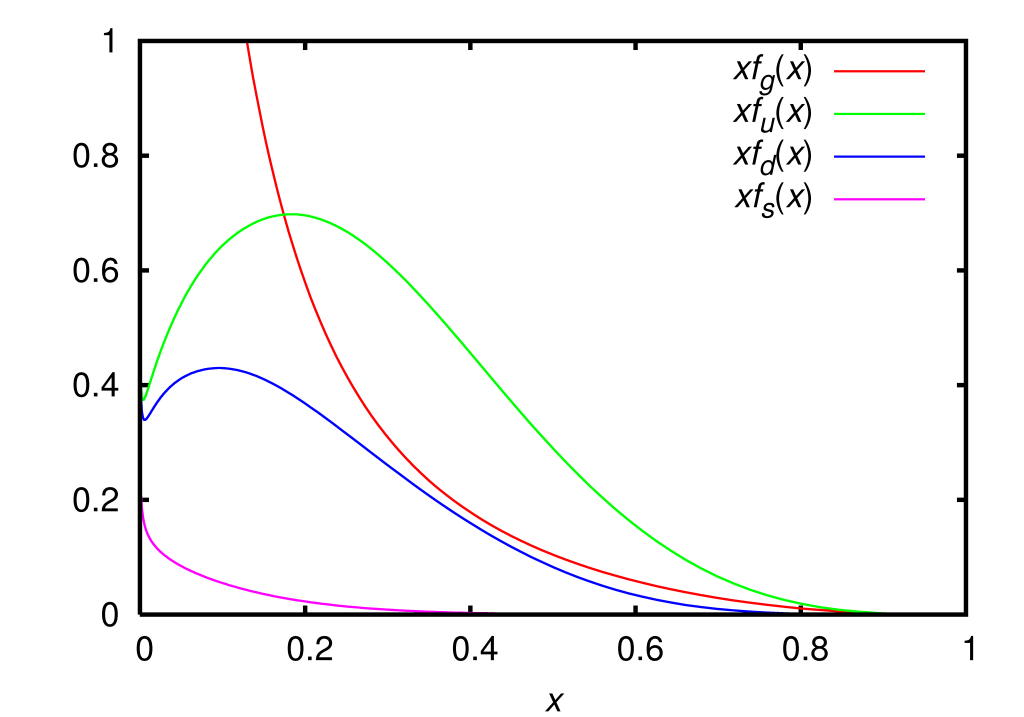
\includegraphics[width=0.45\linewidth]{./gfx/pdfs.png}
\end{figure}

\end{frame}


\begin{frame}
  \frametitle{DGLAP Evolution Equations}

  \begin{itemize}
  \item The DGLAP equations describe how the PDFs evolve with energy
  \end{itemize}

  \begin{equation}
    \frac{\partial f_i(x,Q^2)}{\partial \ln Q^2} = P_{ij}(x, \alpha_s(Q^2)) \otimes f_j(x, Q^2),
  \end{equation}

  \begin{itemize}
  \item $f$ is the PDF, $\alpha_s$ is the strong coupling constant of Quantum Chromodynamics (QCD). 
  \item $P_{ij}$ are the \textit{splitting functions}, which represent probabilities for quarks to emit gluons and vice versa. 
  \item The symbol $\otimes$ represents a convolution product, which is defined as
  \end{itemize}

  \begin{equation}
    [a \otimes b](x) = \int_x^1 \frac{\dd y}{y} a\left( \frac{x}{y} \right) b(y) = \int_x^1 \frac{\dd y}{y} a(y) b\left( \frac{x}{y} \right).
  \end{equation}

\end{frame}


% for this slide, remove most of the stuff and simply mention other methods
% which have some pros and cons, but we want to remain in x since that's real life space
% and we keep the analytical/mathematical structure
\begin{frame}
  \frametitle{Solutions to the DGLAP Equations}

  \begin{itemize}
  \item Due to their mathematical structure, DGLAP cannot in general be solved in a closed form. \\[1cm]
  \item There are many mathematical techniques that can be used, such as the Laplace or Mellin transforms. \\[1cm]
  \item  These map the convolution into a simple algebraic product at the price of transforming back to the original variable.
  \end{itemize}

  \vspace*{3cm}
\end{frame}


\begin{frame}
  \frametitle{Solutions to the DGLAP Equations}

  \begin{itemize}
  \item We work directly in $x$-space ($x$ being the original longitudinal momentum fraction) because this keeps the mathematical/analytical structure of the equations intact.
  \item In addition, it avoids additional transforms to and from some other space.
  \end{itemize}

  \begin{figure}
    \centering
    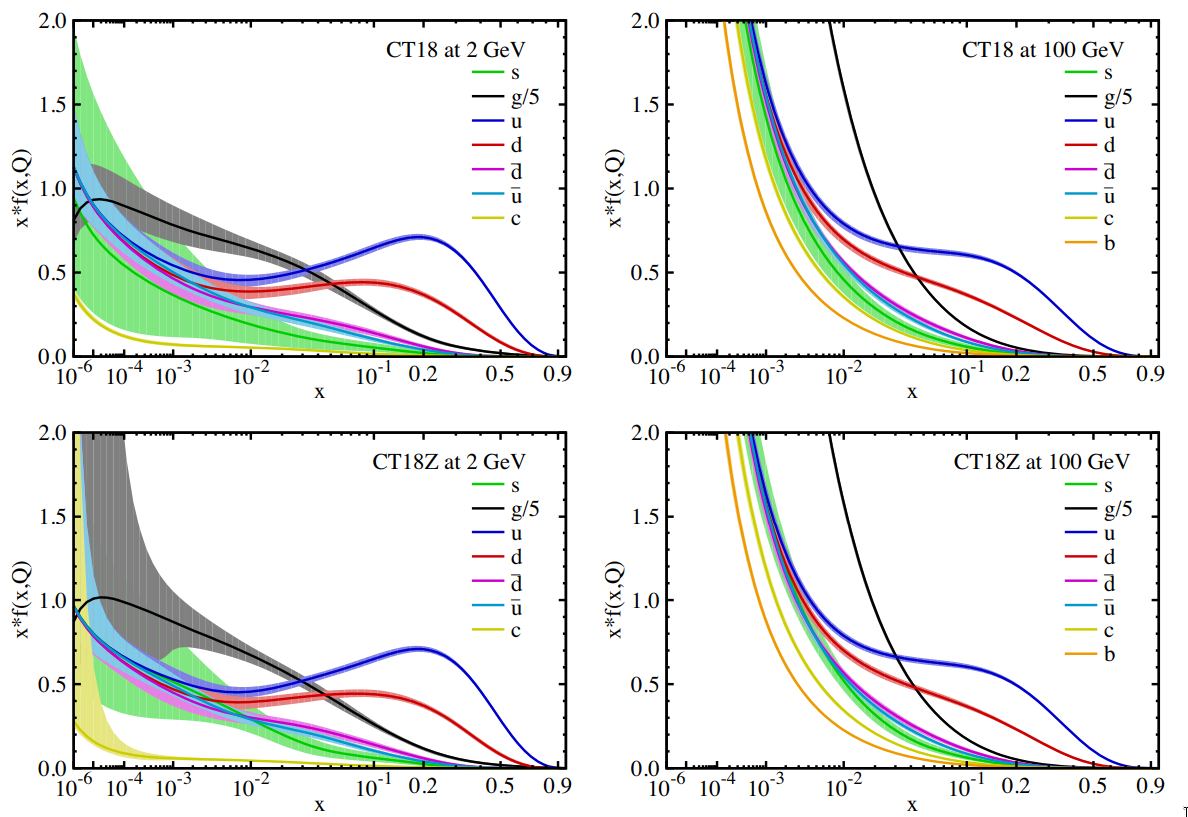
\includegraphics[width=0.6\linewidth]{./gfx/cteq-pdfs.png}
  \end{figure}
  
\end{frame}
  


\begin{frame}
  \frametitle{The Non-singlet Case}

  \begin{itemize}
  \item DGLAP eqns. can be categorized in ``singlet'' and ``non-singlet'' eqns. The singlet eqns. involve matrices, while the non-singlet eqns. involve scalars.
  \item At the lowest order (LO) in perturbation theory, a solution can be given in terms of an ansatz that depends on the initial scale $Q_0$ and a final scale $Q$:
  \end{itemize}

  \begin{equation}
    f(x, Q^2) = \sum_{n=0}^{\infty} \frac{A_n(x)}{n!} \ln^n\left( \frac{\alpha_s(Q^2)}{\alpha_s(Q_0^2)} \right),
  \end{equation}

  \begin{itemize}
  \item The $A_n(x)$ coefficients are determined through recursion relations:
  \end{itemize}

  \begin{equation}
    A_{n+1}(x) = - \frac{2}{\beta_0}[P^{(0)} \otimes A_n] (x).
  \end{equation}
\end{frame}


\begin{frame}
  \frametitle{The Non-singlet Case}

  \begin{itemize}
  \item At the next-to-leading order (NLO) and next-to-next-to-leading order (NNLO) in perturbation theory, the solution accounts for higher order terms. At NLO for example, we have 
  \end{itemize}

  \begin{equation}
    f(x, Q^2) = \sum_{n=0}^{\infty}\sum_{s=0}^n \frac{B_n^s(x)}{n!(s-n)!} \ln^n \left( \frac{\alpha_s}{\alpha_0} \right) \ln^{s-n}\left( \frac{4\pi\beta_0 + \alpha_s\beta_1}{4\pi\beta_0 + \alpha_0\beta_1} \right),
  \end{equation}

  \begin{itemize}
  \item where the $B_s^n(x)$ coefficients satisfy more complicated recursion relations (see Cafarella, Coriano, Guzzi, Nucl.Phys.B 748 (2006)).
  \item {\bf Our goal is to extend this procedure to N$^3$LO in QCD}.  
  \end{itemize}
\end{frame}


\begin{frame}
  \frametitle{The Singlet Case}

  \begin{itemize}
  \item For the singlet case, we consider a solution that can be written as 
  \end{itemize}

  \begin{equation}
    \vv{f}(x, Q^2) = \left[ 1 + \sum_{k=0}^{\kappa} \alpha_s^k \vv{U}_k \right] \otimes \vv{L} \otimes \left[ 1 + \sum_{k=0}^{\kappa} \alpha_0^k \vv{U}_k \right]^{-1} \otimes \vv{f}(x, Q_0^2)
  \end{equation}

  \begin{itemize}
  \item $\vv{U}_k$ are matrices that depend on the splitting functions, and $\vv{L}$ is defined as
  \end{itemize}

  \begin{equation}
    \vv{L} = \left( \frac{\alpha_s(Q)}{\alpha_s(Q_0)} \right)^{-2 P^{(0)}/\beta_0}
  \end{equation}
  
  \begin{itemize}
  \item The Singlet case is more challenging due to the matrix nature of the problem.
  \end{itemize}
\end{frame}


\begin{frame}
  \frametitle{Current Progress}

  \begin{itemize}
  \item We are currently including the most up-to-date version of the splitting functions into our calculation/code.
  
  \item A previous implementation of the algorithm (\textsc{Candia}, Cafarella, Coriano, Guzzi, CPC (2008)) was written in C. 
  It has now been upgraded to C++ with a few minor optimizations. 
  
  Once the new ingredients are added we will release \textsc{Candia-v2} along with a publication in a peer-review journal. 
  \item On the next slide is an example plot for the current version of the algorithm.
  \end{itemize}
\end{frame}


\begin{frame}
  \frametitle{Example Outputs: $u$ quark Distribution}

  \begin{figure}
    \centering
    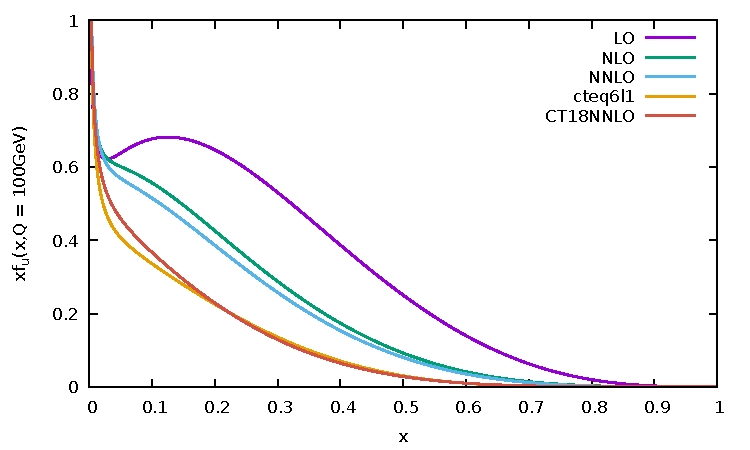
\includegraphics[width=0.9\linewidth]{./gfx/u-new.pdf}
  \end{figure}

  % yellow for CT18NNLO should be changed
\end{frame}



\begin{frame}
  \frametitle{Conclusions}

  \begin{itemize}
  \item This project is of high importance for the next precision frontier of hadron collider phenomenology. 
  \item We are going to extend \textsc{Candia} to N$^3$LO to match the new required precision standards for LHC phenomenology.
  \item Additional efforts will go in improving the CPU turnaround time and efficiency of the numerical implementation.
  \item Results will be published in a peer-reviewed journal and \textsc{Candia-v2} will be made publicly available.
  \end{itemize}
\end{frame}


\end{document}

%%% Local Variables:
%%% mode: LaTeX
%%% TeX-master: t
%%% End:
